%#!ptex2pdf -l -u -ot '--synctex=1 --shell-escape' template
%\documentclass[uplatex]{jsarticle}
\documentclass[uplatex]{ujreport}
\usepackage{booktabs}
\usepackage{amsmath}
\usepackage{amssymb}
\usepackage{psfrag}
\usepackage[T1]{fontenc }
\usepackage{pifont}
\usepackage{algorithm}
\usepackage{algorithmic}
\usepackage{amsmath,cases}
\usepackage{here}
\usepackage[dvipdfmx]{graphicx}
\usepackage{url}      %URLの表記に使う\urlコマンドに必要.
\usepackage{enumerate}%enumerate環境で項目を[Step 1.]のような形式に変更するのに利用.


\setlength{\topmargin}{-10mm}
\setlength{\textheight}{23cm}
\setlength{\oddsidemargin}{5mm}
\setlength{\evensidemargin}{5mm}
\setlength{\textwidth}{15cm}

\renewcommand{\tablename}{表}
\renewcommand{\figurename}{図}
%\newcommand{\bs}{\texttt{\symbol{'134}}}
%    \newcommand{\cmd}[1]{\texttt{\def\{{\char`\{}\def\}{\char`\}}\bs#1}}
\newtheorem{thm}{定理}[section]
\newtheorem{prf}{証明}[section]
\usepackage{latexsym}
\def\qed{\hfill $\Box$}

\usepackage[margin=3.25cm]{geometry}
\renewcommand{\bibname}{参考文献}

\begin{document}





%%%%%%%%%%%%%%%%%%%%%%%%%%%%%%%%%%%%%%%%%%%%%%%%%
%表紙
\begin{table}[b]
\begin{center}
{\huge 修\hspace{0.1cm} 士\hspace{0.1cm} 論\hspace{0.1cm} 文}\\[2.5cm]
{\huge 自動車運搬船における \\ 貨物積載プランニングの席割問題}\\[6cm]
{\huge 252001054\qquad 竹田陽}\\[1cm]
{\huge 名古屋大学大学院情報学研究科}\\[0.5cm]
{\huge 数理情報学専攻}\\[0.5cm]
{\huge 2022年1月}\\
\end{center}
\end{table}
%%%%%%%%%%%%%%%%%%%%%%%%%%%%%%%%%%%%%%%%%%%%%%%%%


\thispagestyle{empty}
\clearpage
\newpage
\pagenumbering{roman}
\setcounter{page}{1}


%%%%%%%%%%%%%%%%%%%%%%%%%%%%%%%%%%%%%%%%%%%%%%%%%
%摘要とabstract
\begin{center}
{\LARGE 自動車運搬船における貨物積載プランニングの\\席割問題に対する局所探索法}\\[0.5cm]
\end{center}
\hfill
{\large 252001054\qquad 竹田 陽}\\[0.5cm]
\begin{center}
{\Large \bf 概 要}\\
\end{center}

ある港から複数の港を経由して自動車を積み, 複数の港で自動車を降ろす自動車運搬船における貨物積載について考える. 自動車運搬船に積む自動車の情報が与えられてから実際に自動車が船に積まれるまでに, 席割と呼ばれる注文1つ1つを船内に割り当てる作業と,シミュレーションと呼ばれる席割で決まった車両を1台ずつ詳細に配置する計画を立てる作業の二種類の作業が行われる. 席割作業では船の階層内を一定間隔の大きさに区切ったホールドと呼ばれるスペースに, 与えられた積載自動車リストのどの自動車を何台割り当てるかを決める. シミュレーション作業では席割作業でホールド毎に割り当てられた自動車を, 自動車の向きや空きスペース,作業効率などを考慮してホールド内への配置を決定する. 本研究では,この席割作業とシミュレーション作業の全自動化への第一歩として席割作業に着目し, 短時間かつ効率の良い席割を出力することを目標とする.

席割問題は割当問題として定式化することができ, 特徴的な要件として以下の2つがある. 一点目は自動車を船に積むあるいは船から降ろす際に, 人が自動車を運転して所定の位置まで移動するための通路を確保する必要があることである. このとき既に積んだ自動車が,新たに積むもしくは降ろす自動車の進行経路上にあると, 自動車は割り当てられたホールドと船の出入り口間を移動することができない. 二点目は船全体の荷重バランスを考慮しなければならないことである. 例えば船が海上を進む際に積まれた自動車が船の一部の領域に集中していると, 船が波に揺られたときにそのまま横転してしまう可能性があり非常に危険である.

良い席割の指標について, 海運会社の業務として席割を作成している作業者や自動車を船内のエリアまで運転して運ぶ運転手へのヒアリングを行った.ヒアリングから,積み降ろし時に意図しない自動車を積み下ろすことが起こりにくいこと, 積み降ろしをする港が同じ自動車が船内でまとまって割り当てられていること,運転手が作業をする効率が落ちない程度のスペースが確保されていること, 船のスペースを無駄にしないことに重点を置いていると考えられた. 本研究ではこのような良い席割の指標を考慮した目的関数を設計する.

本研究では,良い席割を作成するための指標や特徴を考慮した数理モデルを提案する.商用の整数計画ソルバー (Gurobi Optimizer) を使用した厳密解法に基づく数理モデルと,局所探索法を用いた近似解法に基づく数理モデルの2種類を提案し,計算時間や精度の比較を行った.また,局所探索における初期解生成に関して,2種類のアプローチを提案する.一つ目は,整数計画問題として定式化したモデルの線形緩和問題を解き,その解を初期解として利用するというものである.二つ目は,積む港と降ろす港が同じ注文をまとめて一つとみなし,整数計画問題を解き解を初期解として利用するというものである.提案した2種類の手法で得られた解と,ランダムに生成した解の3種類を局所探索における初期解として探索を行い,局所探索が終了するまでの計算時間と解の精度の比較を行う.
計算実験の結果,積む港と降ろす港が同じ注文をまとめて整数計画問題を解き初期解として利用する手法が有効であることが確認できた.
また,厳密解法に基づく数理モデルと比べて,局所探索法を用いたモデルを用いることで,解の精度をあまり落とすことなく計算時間を短縮できることを確認した.

\newpage
\begin{center}{\LARGE A local search algorithm for the stowage planning problem for pure car carrier ships }\\[0.5cm]
\end{center}
\hfill {\large 252001054\qquad Kiyoshi Takeda}\\[0.5cm]
\begin{center}
{\large \bf Abstract}\\
\end{center}

We consider the cargo loading of a car carrier ship, for which cars are loaded and unloaded at several ports.
Two kinds of operations called “stowage planning” and “simulation” are carried out after the information of cars to be loaded on a car carrier is given.
In the stowage planning, they decide how many cars from the given list of cars should be assigned to the spaces called holds, which the spaces are obtained by dividing a deck of the ship into certain intervals.
In the simulation work, the cars assigned to each hold in the stowage planning work are determined to be placed in the hold considering the direction of the cars, available space, and work efficiency.
As a first step to automating these tasks, we aim to automate the work of stowage planning.

The stowage planning problem can be formulated as an assignment problem, and there are two characteristic requirements.
The first is that when loading or unloading a car onto or off a ship, it is necessary to secure a passage for a person to drive the car to a certain position.
In this case, if a car already loaded is in the path of a car to be newly loaded or unloaded, the car cannot move between the assigned hold and the entrance of the ship.
Secondly, the load balance of the entire ship must be considered.
For example, if the loaded cars are concentrated in some areas of the ship as the ship moves through the sea, it is very dangerous that the ship may roll over when it is rocked by waves.

From the interviews, we have confirmed that it is important not to cause unintended cars to be unloaded during loading and unloading, that cars with the same port of loading and unloading are placed close to each other on the ship, that there is enough space for the driver to work efficiently, and that the space on the ship is not wasted. In this study, we design an objective function that takes these indicators of good stowage planning into account.

In this study, we propose a mathematical model that takes into account indicators and features for creating a good stowage plan. Two types of mathematical models are proposed: one is based on an exact solution method using an integer programming solver, and the other is based on an approximate solution method using a local search method, and we compare the computation time and accuracy.
We also propose two approaches to generate initial solution. The first one is to solve the linear relaxation problem of the model formulated as an integer programming problem and use the solution as the initial solution. The second approach is to consider all orders with the same loading and unloading ports as a single order, solve the integer programming problem, and use the solution as the initial solution. We compare the computation time and the accuracy of the solution by using the proposed two approaches and a randomly generated solution as the initial solution in the local search.
As a result of computational experiments, the method using the initial solution based on the second approach is effective.
We also confirmed that the model using the local search method can reduce the computation time without losing much accuracy of the solution.




\thispagestyle{empty}
\tableofcontents
\newpage
\setcounter{page}{1}
\pagestyle{plain}
\pagenumbering{arabic}



\chapter{はじめに}
これは卒論や修論のテンプレートです.
卒論や修論を作る前に,書き物に関する基本的な注意点を書いたページ
\footnote{\url{http://www.co.cm.is.nagoya-u.ac.jp/~yagiura/writing/writing.html}}
に書いたことをよく読んでください.
このページには加筆,訂正することがときどきあるので,資料を作るたびに見直してください.

発表のたびに配布資料を書く(あるいは前回の資料に加筆修正する)ことで,
論文のための文章を書くことや\LaTeX を使うことに慣れるとともに,
卒論・修論につながる文章を蓄積していってください.

このテンプレートはあくまでも参考ですので,
フォントサイズや行間等のスタイルを自由に変更してかまいません.

「はじめに」の節ではこの資料で何を書くのかを手短に説明してください.
どのような問題を対象にしてどのような手法を提案し,どのような結果が得られたのかを書くなどです.
また,研究背景についても関連研究の文献を挙げつつ述べましょう.
文献リストの書き方の例を挙げておきます.
\cite{GareyJohnson79}は本,
\cite{MHI13,YIG04}は論文誌の論文,
\cite{IYI05}は国際会議の予稿集の論文,
\cite{JohnsonMcGeoch97}は論文を集めた本やハンドブックに掲載された論文の例です.

必要な情報を
順序よく(つまり後ろを見ないと分からないことが出て来たりしないように),
明確に(曖昧さなく厳密に),
コンパクトに(冗長な表現を無くして手短に)書くよう心がけましょう.


構成は研究テーマや書きたいことによって様々ですが,
例えばある問題に対するアルゴリズムを提案して,
その効果を計算実験によって検証するようなテーマであれば,はじめにの節ののち,
問題の説明,提案手法の説明,計算実験の紹介,まとめという構成がしばしば用いられます.
以下の節ではそのような説明を書く際によく利用する書式や書くべきことの例をいくつか示しておきます.
\chapter{問題設定}\label{definition}

複数の港を経由し, 自動車を輸送する運搬船を想定する. 例えば乗用車100台を港Aから港B, トラック30台を港Cから港Dというような各注文を, 運搬船の階層毎に一定の広さで区切られたスペースへの割当を計画する.この作業を席割作業(stowage plan)\cite{stowage}という. 本稿では複数の種類がある運搬船のなかで,単純な船の構造データを用いて実験する. また実際の席割業務では積載する自動車の種類が多様であり, ブルードーザーやショベルカーなどの建機は高さや重さが乗用車とは大きく異なるので特定の領域にしか収容出来ないという問題がある. これに対し本稿では作業自動化の初期段階として,自動車を全て乗用車とし, 船内の任意領域においてどの自動車も積載が可能と言う条件で席割を作成する. この章では一般的な船への自動車積載における専門用語の定義, 席割作業における入力情報や出力情報の説明をする.

\section{用語定義}
本研究で扱う船の航海等に関する専門用語の定義をする.

\begin{itemize}

\item 席割 \\
注文一つ一つを船のホールド割り当てる作業.

\item シミュレーション \\
席割で決まった自動車を一台ずつホールド内の領域に貼り付ける作業.

\item  プランナー \\
席割やシミュレーションを考える作業者.

\item  ギャング\\
港で自動車をホールドまで運転して積み降ろしをする作業者.

\item デッキ \\
船の内部の階層.

\item ホールド \\
各デッキ内を一定間隔の領域で仕切られた空間.

\item ランプ \\
上下デッキに移動するために各デッキの特定ホールドについているスロープ.

\item 注文 \\
乗用車100台を港Aから港Bへ輸送, トラック30台を港Cから港Dへ輸送というような積載自動車の情報とそれらの積み地と揚げ地に関する情報.

\item 積み地 \\
注文における自動車を積む港.

\item 揚げ地 \\
注文における自動車を降ろす港.

\item  RT (revenue ton) \\
基準となる車一台の面積に対する各注文の車の面積の割合. 本研究ではこれを資源要求量として扱う$[4]$.

\item ユニット数 \\
各注文に含まれる自動車の台数.

\end{itemize}

%2ページ

\section{入力情報}
本研究で扱う二種類の情報について述べる.
\begin{itemize}

\item 注文情報 \\
本稿では注文内に含まれる情報のうち注文番号, 積み地と揚げ地, ユニット数, 積載自動車のRT, 自動車の重量情報を扱う.

\item 船体情報 \\
輸送に使う船のデッキやホールド番号, 各ホールドへアクセスすために通るホールドや各ホールドの許容収容量などの船の内部構造に関する情報.

\end{itemize}

入力情報のうち注文情報の例を表\ref{table21}に, 船体情報の例を表\ref{table22}に示す. \\

\begin{table}[htbp]
\tabcolsep = 15pt
\renewcommand{\arraystretch}{0.8}
\caption{注文情報の例}
\label{table21}
\begin{center}
\begin{tabular}{rccrrr} \hline
注文番号 & 積み地 & 揚げ地 & ユニット数 & RT & 重さ(kg) \\ \hline
1 & 港1 & 港3 & 20 & 1.43 & 1480 \\
2 & 港1 & 港3 & 200 & 1.51 & 2680 \\
3 & 港1 & 港4 & 50 & 1.57 & 2580 \\
4 & 港2 & 港3 & 14 & 1.67 & 1720 \\
5 & 港2 & 港4 & 150 & 1.18 & 1810 \\
\hline
\end{tabular}
\end{center}
\end{table}

\begin{table}[htbp]
\centering
\tabcolsep = 15pt
\renewcommand{\arraystretch}{0.8}
\caption{船体情報の例}
\label{table22}
\begin{center}
\begin{tabular}{rrrr} \hline
デッキ番号 & ホールド番号 & 収容量 \\ \hline
1 & 2 & 80  \\
1 & 3 & 100  \\
2 & 1 & 25  \\
2 & 2 & 100 \\
2 & 3 & 150  \\
3 & 1 & 30 \\
3 & 2 & 200 \\
3 & 3 & 200 \\
\hline
\end{tabular}
\end{center}
\end{table}

%3ページ

\newpage

\section{出力}
入力情報を元に様々な条件を考慮して注文番号1番を2デッキ2ホールドに30台中30台割り当てるというような席割を出力する. 出力結果の例を表\ref{table23}に示す. \\

\begin{table}[htbp]
\centering
\tabcolsep = 15pt
\renewcommand{\arraystretch}{0.8}
\caption{出力結果の例}
\label{table23}
\begin{center}
\begin{tabular}{rcccrr} \hline
注文番号 & 積み地 & 揚げ地 & 割当先ホールド & 積載台数 & ユニット数 \\ \hline
1 & 港1 & 港3 & 3階-1 & 30 & 30 \\
2 & 港1 & 港3 & 2階-2 & 40 & 200 \\
2 & 港1 & 港3 & 3階-2 & 60 & 200 \\
2 & 港1 & 港3 & 3階-3 & 60 & 200 \\
3 & 港1 & 港4 & 2階-3 & 50 & 50 \\
4 & 港2 & 港3 & 2階-1 & 14 & 14 \\
5 & 港2 & 港3 & 1階-2 & 67 & 150 \\
5 & 港2 & 港4 & 1階-3 & 83 & 150 \\
\hline
\end{tabular}
\end{center}
\end{table}

%4ページ

\chapter{定式化}\label{formulation}

この章では各注文に含まれる自動車を, どのホールドに何台割り当てるかを最適化する複数の数理モデルを提案する. モデルは二種類ありプランナー側の要望を全て目的関数で表したモデルSP1-1と, 求解時間削減のため一部の目的関数を制約化したモデルSP1-2を紹介する.

\section{記号の定義}
本研究における変数と定数記号の定義をする. 本研究の変数の定義を表\ref{table31}に, 定数の定義を表\ref{table32}に記載する. \\

\begin{table}[htb]
\caption{変数の定義}
\begin{center}
\label{table31}
\begin{tabular}{cp{35em}} \hline
変数 & \hspace{2.0em}変数の説明 \\ \hline

$v_{ij}$ &
\begin{tabular}{l}
\hspace{1.4em}注文$j$をホールド$i$に$n$台割り当てるとき$v_{ij} = n$ \\
\end{tabular} \\ \hline

$x_{ij}$ &
\begin{tabular}{l}
\hspace{1.4em}注文$j$をホールド$i$に割り当てるとき$x_{ij} = 1$ \\
\hspace{1.4em}そうでないとき$x_{ij} = 0$ \\
\end{tabular} \\ \hline

$n_{it}$ &
\begin{tabular}{l}
\hspace{1.4em}港$t$でのホールド$i$の残容量が$b'_i$のとき$n_{it} =  b'_i$ \\
\end{tabular} \\ \hline

$c_{ij}$ &
\begin{tabular}{l}
\hspace{1.4em}ホールド$i$に大きい注文$j$を100台以下に分割して積むとき$c_{ij} = 1$ \\
\hspace{1.4em}そうでないとき$c_{ij} = 0$ \\
\end{tabular} \\ \hline

$c_{i_1i_2j}^1$ &
\begin{tabular}{l}
\hspace{1.4em}ホールドペア$(i_1, i_2)$に \\
\hspace{1.4em}1.大きい注文$j_1$を分割して積むとき$c_{i_1i_2j_1}^1 = p_{\rm{large}}^{\rm{c1}}$ \\
\hspace{1.4em}2.小さい注文$j_2$を分割して積むとき$c_{i_1i_2j_2}^1 = p_{\rm{small}}^{\rm{c1}}$ \\
\hspace{1.4em}3.それら以外のとき$c_{i_1i_2j}^1 = 0$ \\
\end{tabular} \\ \hline

$c_{i_1i_2j}^2$ &
\begin{tabular}{l}
\hspace{1.4em}分割した大きい注文$j_1$を \\
\hspace{1.4em}1.隣のホールドペア$(i_1, i_2)$に積むとき$c_{i_1i_2j_1}^2 = n\_p_{\rm{large}}^{\rm{c2}}$ \\
\hspace{1.4em}2.同デッキの隣ではないホールドペア$(i_1, i_2)$に積むとき$c_{i_1i_2j_2}^2 = s\_p_{\rm{large}}^{\rm{c2}}$ \\
\hspace{1.4em}分割した小さい注文$j_2$を \\
\hspace{1.4em}3.隣のホールドペア$(i_1, i_2)$に積むとき$c_{i_1i_2j_2}^2 = n\_p_{\rm{small}}^{\rm{c2}}$ \\
\hspace{1.4em}4.同デッキの隣ではないホールドペア$(i_1, i_2)$に積むとき$c_{i_1i_2j_2}^2 = s\_p_{\rm{small}}^{\rm{c2}}$ \\
\hspace{1.4em}5.それら以外のとき$c_{i_1i_2j}^2 = 0$ \\
\end{tabular} \\ \hline

$m_{it}$ &
\begin{tabular}{l}
\hspace{1.4em}ホールド$i$が港$t$で作業効率充填率を超えているとき$m_{it} = 1$ \\
\hspace{1.4em}そうでないとき$m_{it} = 0$ \\
\end{tabular} \\ \hline

$m_{ijt}$ &
\begin{tabular}{l}
\hspace{1.4em}港$t$で注文$j$をホールド$i$から積み降ろしを行う際, $n$個の通過ホールドで \\
\hspace{1.4em}作業効率充填率を超えそこを$v$台車が通るとき$m_{ijt} = vn$ \\
\end{tabular} \\ \hline

\end{tabular}
\end{center}
\end{table}

%5ページ

\begin{table}[htb]
\begin{center}
\begin{tabular}{cp{35em}} \hline

$k_{it}^1$ &
\begin{tabular}{l}
\hspace{1.4em}ホールド$i$が港$t$で許容充填率を超えているとき$k_{it}^1= 1$ \\
\hspace{1.4em}そうでないとき$k_{it}^1 = 0$ \\
\end{tabular} \\ \hline

$k_{it}^2$ &
\begin{tabular}{l}
\hspace{1.4em}ホールド$i$の残容量が1RTを超えているとき$k_{it}^2 = 1$ \\
\hspace{1.4em}そうではないとき$k_{it}^2 = 0$ \\
\end{tabular} \\ \hline

$k_{it}^3$ &
\begin{tabular}{l}
\hspace{1.4em}ホールド$i$が港$t$で許容充填率を超えてそれよりの奥のホールドの中で1RT \\
\hspace{1.4em}を超えたホールドが$n$個あるとき$k_{it}^3 = n$ \\
\hspace{1.4em}ホールド$i$が港$t$で許容充填率を超えていないとき$k_{it}^3 = 0$ \\
\end{tabular} \\ \hline

$y_{it}^{\rm{keep}}$ &
\begin{tabular}{l}
\hspace{1.4em}ホールド$i$の中で港$t$を通過する注文があるとき$y_{it}^{\rm{keep}} = 1$ \\
\hspace{1.4em}そうでないとき$y_{it}^{\rm{keep}} = 0$ \\
\end{tabular} \\ \hline

$y_{it_1t_2}$ &
\begin{tabular}{l}
\hspace{1.4em}ホールド$i$の中で港$t_1$で積んで港$t_2$で降ろす注文があるとき$y_{it_1t_2} = 1$ \\
\hspace{1.4em}そうでないとき$y_{it_1t_2} = 0$ \\
\end{tabular} \\ \hline

$z_{it_1t_2}$ &
\begin{tabular}{l}
\hspace{1.4em}ホールド$i$の中で港$t_2$を通過する注文があり港$t_2$で降ろす注文の中に港$t_1$ \\
\hspace{1.4em}で積んだ注文があるとき$z_{i_1i_2t_1t_2} = 1$ \\
\hspace{1.4em}そうでないとき$z_{it_1t_2} = 0$ \\
\end{tabular} \\ \hline

$y_{i_1i_2t}^{\rm{load}}$ &
\begin{tabular}{l}
\hspace{1.4em}隣接ホールドペア$(i_1, i_2)$の中で港$t$で積む注文があるとき$y_{i_1i_2t}^{\rm{load}} = 1$ \\
\hspace{1.4em}そうでないとき$y_{i_1i_2t}^{\rm{load}} = 0$ \\
\end{tabular} \\ \hline

$y_{i_1i_2t}^{\rm{keep}}$ &
\begin{tabular}{l}
\hspace{1.4em}隣接ホールドペア$(i_1, i_2)$の中で港$t$を通過する注文があるとき$y_{i_1i_2t}^{\rm{keep}} = 1$ \\
\hspace{1.4em}そうでないとき$y_{i_1i_2t}^{\rm{keep}} = 0$ \\
\end{tabular} \\ \hline

$y_{i_1i_2t}^{\rm{dis}}$ &
\begin{tabular}{l}
\hspace{1.4em}隣接ホールドペア$(i_1, i_2)$の中で港$t$で降ろす注文があるとき$y_{i_1i_2t}^{\rm{dis}} = 1$ \\
\hspace{1.4em}そうでないとき$y_{i_1i_2t}^{\rm{dis}} = 0$ \\
\end{tabular} \\ \hline

$z_{i_1i_2t}^1$ &
\begin{tabular}{l}
\hspace{1.4em}隣接ホールドペア$(i_1, i_2)$の中で港$t$を通過する注文と積む注文があるとき \\
\hspace{1.4em}$z_{i_1i_2t}^1 = 1$ \\
\hspace{1.4em}そうでないとき$z_{i_1i_2t}^1 = 0$ \\
\end{tabular} \\ \hline

$z_{i_1i_2t}^2$ &
\begin{tabular}{l}
\hspace{1.4em}隣接ホールドペア$(i_1, i_2)$の中で港$t$を通過する注文と降ろす注文があるとき \\
\hspace{1.4em}$z_{i_1i_2t}^2 = 1$ \\
\hspace{1.4em}そうでないとき$z_{i_1i_2t}^2 = 0$ \\
\end{tabular} \\ \hline

\end{tabular}
\end{center}
\end{table}

\begin{table}[htb]
\caption{定数の定義}
\begin{center}
\label{table32}
\begin{tabular}{cp{35em}} \hline
定数 & \hspace{2.0em}定数の説明  \\ \hline

$T$ &
\begin{tabular}{l}
\hspace{1.4em}港の集合
\end{tabular} \\ \hline

$T^{\rm{c}}$ &
\begin{tabular}{l}
\hspace{1.4em}チェックポイント港の集合
\end{tabular} \\ \hline

$L$ &
\begin{tabular}{l}
\hspace{1.4em}積み地の集合
\end{tabular} \\ \hline

$D$ &
\begin{tabular}{l}
\hspace{1.4em}揚げ地の集合
\end{tabular} \\ \hline

$K$ &
\begin{tabular}{l}
\hspace{1.4em}船のデッキの集合
\end{tabular} \\ \hline

$J$ &
\begin{tabular}{l}
\hspace{1.4em}注文の集合
\end{tabular} \\ \hline

$J^{\rm{large}}$ &
\begin{tabular}{l}
\hspace{1.4em}ユニット数100台以上の大きい注文の集合
\end{tabular} \\ \hline

$J^{\rm{small}}$ &
\begin{tabular}{l}
\hspace{1.4em}ユニット数100台以下の小さい注文の集合
\end{tabular} \\ \hline

$J_{t}^{\rm{load}}$ &
\begin{tabular}{l}
\hspace{1.4em}港$t$で載せる注文の集合
\end{tabular} \\ \hline

$J_{t}^{\rm{keep}}$ &
 \begin{tabular}{l}
\hspace{1.4em}港$t$を通過する注文の集合
\end{tabular} \\ \hline

$J_{t}^{\rm{dis}}$ &
\begin{tabular}{l}
\hspace{1.4em}港$t$で降ろす注文の集合
\end{tabular} \\ \hline

\end{tabular}
\end{center}
\end{table}

%6ページ

\begin{table}[htb]
\begin{center}
\begin{tabular}{cp{35em}} \hline

$J_{t}^{\rm{lk}}$ &
\begin{tabular}{l}
\hspace{1.4em}$J_{t}^{\rm{load}}$と$J_{t}^{\rm{keep}}$の和集合
\end{tabular} \\ \hline

$J_{t}^{\rm{ld}}$ &
\begin{tabular}{l}
\hspace{1.4em}$J_{t}^{\rm{load}}$と$J_{t}^{\rm{dis}}$の和集合
\end{tabular} \\ \hline

$I$ &
 \begin{tabular}{l}
\hspace{1.4em}船のホールドの集合
\end{tabular} \\ \hline

$I^{\rm{lamp}}$ &
\begin{tabular}{l}
\hspace{1.4em}ランプがついているホールドの集合
\end{tabular} \\ \hline

$ I^{\rm{next}}$ &
\begin{tabular}{l}
\hspace{1.4em}隣同士のホールドペアの集合
\end{tabular} \\ \hline

$ I^{\rm{same}}$ &
\begin{tabular}{l}
\hspace{1.4em}同一デッキ内にあるホールドペアの集合
\end{tabular} \\ \hline

$ \overline{I}$ &
\begin{tabular}{l}
\hspace{1.4em}隣接しているホールドペアの集合
\end{tabular} \\ \hline

$ I^{\rm{num}}$ &
 \begin{tabular}{l}
\hspace{1.4em}船のホールド総数
\end{tabular} \\ \hline

$I_{k}^{\rm{deck}}$  &
 \begin{tabular}{l}
\hspace{1.4em}デッキ$k$のホールドの集合
\end{tabular} \\ \hline

$I_{i}^{\rm{back}}$  &
 \begin{tabular}{l}
\hspace{1.4em}ホールド$i$よりも奥のホールドの集合
\end{tabular} \\ \hline

$I^{*}_i$ &
 \begin{tabular}{l}
\hspace{1.4em}ホールド$i$に辿り着くまでに通るホールドの集合
\end{tabular} \\ \hline

$u_{j}$ &
\begin{tabular}{l}
\hspace{1.4em}注文$j$に含まれる自動車の台数
\end{tabular} \\ \hline

$g_{j}$ &
\begin{tabular}{l}
\hspace{1.4em}注文$j$における自動車一台の重量
\end{tabular} \\ \hline

$a_{j}$ &
\begin{tabular}{l}
\hspace{1.4em}注文$j$における自動車一台のRT
\end{tabular} \\ \hline

$b_{i}$ &
\begin{tabular}{l}
\hspace{1.4em}ホールド$i$の総面積
\end{tabular} \\ \hline

$\delta_{i}^{\rm{h}}$ &
\begin{tabular}{l}
\hspace{1.4em}船の横方向のホールド$i$の重み
\end{tabular} \\ \hline

$d^{\rm{s}}$ &
\begin{tabular}{l}
\hspace{1.4em}最大許容デッドスペース
\end{tabular} \\ \hline

$f_1^{\rm{h}}$ &
\begin{tabular}{l}
\hspace{1.4em}船の横方向の後方許容値
\end{tabular} \\ \hline

$f_2^{\rm{h}}$ &
\begin{tabular}{l}
\hspace{1.4em}船の横方向の前方許容値
\end{tabular} \\ \hline

$\delta_{i}^{\rm{v}}$ &
\begin{tabular}{l}
\hspace{1.4em}船の縦方向のホールド$i$の重み
\end{tabular} \\ \hline

$f^{\rm{v}}$ &
\begin{tabular}{l}
\hspace{1.4em}船の縦方向の上方許容値
\end{tabular} \\ \hline

$ \overline{q}_{i}$ &
\begin{tabular}{l}
\hspace{1.4em}ホールド$i$における許容充填率
\end{tabular} \\ \hline

$ \overline{q}^{\rm{s}}_{i}$ &
\begin{tabular}{l}
\hspace{1.4em}ホールド$i$における作業効率充填率
\end{tabular} \\ \hline

$\delta_i^{\rm{n}}$ &
\begin{tabular}{l}
\hspace{1.4em}ホールド$i$の残RT利得
\end{tabular} \\ \hline

$p^{\rm{c}}$ &
\begin{tabular}{l}
\hspace{1.4em}変数$c_{ij}$のペナルティ重み
\end{tabular} \\ \hline

$p^{\rm{k}}$ &
\begin{tabular}{l}
\hspace{1.4em}変数$k_{it}^3$のペナルティ重み
\end{tabular} \\ \hline

$p^{\rm{z}}$ &
\begin{tabular}{l}
\hspace{1.4em}変数$z_{it_1t_2}$のペナルティ重み
\end{tabular} \\ \hline

$p^{\rm{z}}_1$ &
\begin{tabular}{l}
\hspace{1.4em}変数$z_{i_1i_2t_1t_2}^1$のペナルティ1
\end{tabular} \\ \hline

$p^{\rm{z}}_2$ &
\begin{tabular}{l}
\hspace{1.4em}変数$z_{i_1i_2t_1t_2}^2$のペナルティ
\end{tabular} \\ \hline

$p_{\rm{large}}^{\rm{c1}}$ &
\begin{tabular}{l}
\hspace{1.4em}大きい注文の変数$c_{i_1i_2j}^1$のペナルティ
\end{tabular} \\ \hline

$p_{\rm{small}}^{\rm{c1}}$ &
\begin{tabular}{l}
\hspace{1.4em}小さい注文の変数$c_{i_1i_2j}^1$のペナルティ
\end{tabular} \\ \hline

$p_{\rm{large}}^{\rm{sc2}}$ &
\begin{tabular}{l}
\hspace{1.4em}大きい注文の変数$c_{i_1i_2j}^2$の緩和量1
\end{tabular} \\ \hline

$p_{\rm{large}}^{\rm{nc2}}$ &
\begin{tabular}{l}
\hspace{1.4em}大きい注文の変数$c_{i_1i_2j}^2$の緩和量2
\end{tabular} \\ \hline

$p_{\rm{small}}^{\rm{sc2}}$ &
\begin{tabular}{l}
\hspace{1.4em}小さい注文の変数$c_{i_1i_2j}^2$の緩和量1
\end{tabular} \\ \hline

$p_{\rm{small}}^{\rm{nc2}}$ &
\begin{tabular}{l}
\hspace{1.4em}小さい注文の変数$c_{i_1i_2j}^2$の緩和量2
\end{tabular} \\ \hline

$w_1$ &
\begin{tabular}{l}
\hspace{1.4em}目的関数(a)の重み
\end{tabular} \\ \hline

$w_2$ &
\begin{tabular}{l}
\hspace{1.4em}目的関数(b)の重み
\end{tabular} \\ \hline

$w_3$ &
\begin{tabular}{l}
\hspace{1.4em}目的関数(c)の重み
\end{tabular} \\ \hline

$w_4$ &
\begin{tabular}{l}
\hspace{1.4em}目的関数(d)の重み
\end{tabular} \\ \hline

$w_5$ &
\begin{tabular}{l}
\hspace{1.4em}目的関数(e)の重み
\end{tabular} \\ \hline

$w_6$ &
\begin{tabular}{l}
\hspace{1.4em}目的関数(f)の重み
\end{tabular} \\ \hline

\end{tabular}
\end{center}
\end{table}

%7ページ

\clearpage


\section{制約}
モデルSP1-1で考慮する本研究の独自の制約について記す.  \\

\textgt{(a)自動車移動経路に関する制約} \\
 ある港において注文が運搬船内の特定のホールドで積み降ろしがあるとき, 自動車がホールドへ到達するためには船の入口とホールドの間で通過する任意のホールドに対して自動車が通るための道を作る必要がある. 従って, 本研究では各ホールドに対して自動車の移動通路が十分確保出来る許容充填率を定義し, 任意の港で各ホールドに注文を積むときや各ホールドから注文を降ろすときには, 入口とそのホールドの間で通過する全てのホールドで, その港における充填率が許容充填率以下であることが必要である. 本研究ではこれを制約にすることで, 現実的に自動車の積み降ろしが不可能になる席割を禁止する. \\

\textgt{(b)船内重量バランスに関する制約} \\
 運搬船で自動車を運ぶ際に船の前方や後方へ自動車を詰め込みすぎたり, 船の上方へ自動車を詰め込みすぎると船が傾いたときにバランスを崩しそのまま横転してしまう可能性がある$[5]$. 本研究ではこの問題を考慮するため, 過去10回分の航海データを解析することによりその航海内での運搬船の重量バランスを数値化した. その結果得られた10回分の航海データの中で船内重量バランスが最も偏ったときを閾値とし, 運搬船の上下方向と前後方向それぞれに対して, 各港において運搬船から降ろす注文を全て降ろしたとき, または港で積む注文を全て積んだときについて船内重量バランスが閾値を超えてしまうような自動車の割当を禁止する.

\section{目的関数}
席割に関するプランナーやギャングとの意見交換や席割作業を実際に体験することで, プランナーは席割を考える上で注文の積み間違えや降ろし間違えが起こらないような席割や, ギャングにとって効率が良いような席割を目指していることが分かった. 本研究では, このような席割を実現するための6つの目的関数のパラメータを提案する. \\

\textgt{(a)一つのホールド内の降ろし地を揃える} \\
 ある港においてホールドから注文を降ろす場合, 同じホールド内に揚げ地の異なる注文が複数存在していると注文の降ろし間違いが発生する可能性がある. 本研究では揚げ地において各ホールド内で揚げ地を通過する注文があるときに, その揚げ地で降ろす注文があるとペナルティが発生する.  またこのとき更に降ろす注文の中で積み地が異なる注文が複数含まれていたとする. この場合席割作業の次にシミュレーション作業を行う際, プランナーは降ろし間違えを防ぐため揚げ地が同じ注文は出来るだけホールド内の一つの領域に行き渡るようにホールド内のスペース配分などを考慮しなければならない. このようなプランナーの負担を考え, この場合は降ろす注文の中に含まれる相異なる積み地の分だけ更にペナルティが加算される. \\

%8ページ

\textgt{(b)船内で注文の積み降ろし地を揃える} \\
 ギャング達とのヒアリングで, 積み間違いや降ろし間違いを防ぐためになるべく積み地や揚げ地が同じ注文は船内の同じ場所で固めておきたいという要望があった. 本研究ではこの要望に応えるために隣接ホールドペアを用意した. 隣接ホールドペアとは隣同士に位置するホールド同士のペアと, ランプで繋がったホールド同士のペアのことを指す. 各隣接ホールドペアに対して積み地や揚げ地が異なっている注文が存在していると, その数分ペナルティが発生する. ただし, プランナーの要望で積み地がバラけてしまっても, 揚げ地はなるべく固めたいとの意見をいただいたため, 目的関数(b)のペナルティ重みは揚げ地のペナルティ重みを積み地よりも重く設定している. \\

\textgt{(c)作業効率充填率を考慮する} \\
 ある港で注文の積み降ろしのために自動車をホールドから出すときやホールドに自動車を入れるときに, そのホールドと入口の間で通過するホールドにはその港を通過する注文が一定数存在する. この注文がホールドの領域に対して一定量以上の場合, プランナーはそのホールドを自動車が通れるための道を作る必要がありホールド内における自動車のスペース配分を考える必要がある. またギャングは作られた道に自動車を通さなければいけないため, 自動車の移動に慎重になり全体の作業効率が落ちる可能性が高い. 本研究ではこのように作業効率が落ちないための各ホールド毎の作業効率充填率を設定し, これを上回ったホールドを自動車が通過する場合にペナルティが発生する. \\

\textgt{(d)デッドスペースを作らない} \\
 注文の合計資源要求量が船の合計収容量より十分小さい場合, 特定のホールドに空きスペースが出来る. このスペースが入口付近にあれば追い積みという港での突然の追加注文を積むことに対応出来るが, 空きスペースが出来たホールドに到達するまでに通るホールドが許容充填率を上回っている場合は, このスペースに追い積みをすることは出来ない. このような空きスペースのことをデッドスペースと言う. 目的関数(d)ではランプで繋がった船のホールドが許容充填率を超え特定デッキ間の移動ができない状態になったとき, そのホールドよりも奥にあるホールドの中で, 指定された最大許容デッドスペースよりも大きいデッドスペースがあるホールドが存在するときに大きいペナルティが発生する. \\

\textgt{(e)残容量をなるべく入口付近に寄せる} \\
 船の入口に近いホールドにまだ自動車を入れることのできるスペースがあると船への追い積みに対応できる. また, 研究で扱う船は追い積みに対応しやすい5デッキに残容量をなるべく残したいとのプランナーから要望があった. 目的関数(e)では, 積載自動車を全て積み終わる最後の積み地をチェックポイントとし, チェックポイントで5デッキや入口に近いホールドに対して残容量が多いほど全体目的関数のペナルティを減らす利得が発生する. \\

%9ページ

\textgt{(f)注文の分割ルールを守る} \\
 注文の資源要求量は, あるホールドに割り当てる注文の車のユニット数とその自動車一台のRTの積で表現する. 従って注文に含まれる自動車のユニット数が膨大な場合, どのホールドにもその注文を割り当てることが出来ないという問題が発生する. この場合は注文の容量を適当な大きさに分割して複数ホールドへ収容する必要がある. 実際の席割プランニング上ではこの場合, まず注文に含まれる合計ユニット数が100台以上の大きい注文と小さい注文に分類する. 小さい注文については, 分割して異なるホールドに入れるとギャングが自動車を積むときに混乱を招きやすいため基本的には分割をすることはないが, 隣りあったホールド同士にちょうど良いスペースがあるときだけは分割してそれぞれのホールドに入れる. 目的関数(f)では小さい注文に関して, 隣り合ったホールド同士以外に分割して注文を入れる場合は大きいペナルティが発生する. 大きい注文については一つのホールドに全てを入れることは不可能なため分割が必要であるが,  100台以下の小さいサイズに分割してしまうとホールドの挿入先が増えてギャングの負担が増えるため, 100台以下で分割した場合はペナルティが発生する. 更に分割した注文を二つの異なるデッキ内のホールドに分割した場合, 同デッキ内の隣接しないホールドに分割した場合, 同デッキ内の隣接ホールドに分割した場合の順に大きいペナルティがかかる. \\

\section{定式化}
定式化を行う.

\begin{center}
\begin{align}
&\textrm{min} \hspace{1.0em} {w_1 p^{\rm{z}} \sum_{i \in I} \sum_{t_1 \in L}  \sum_{t_2 \in D} {z_{it_1t_2}}}
+ {w_2 \sum_{i_1 \in I} \sum_{i_2 \in I} ( p_1^{\rm{z}} \sum_{t_1 \in L} {z_{i_1i_2t_1}^1} + p_2^{\rm{z}} \sum_{t_2 \in D} {z_{i_1i_2t_2}^2} )} \notag \\
&\hspace{2.45em} + {w_3 \hspace{0.1em} \sum_{i \in I} \sum_{j\in J} \sum_{t \in T}  {m_{ijt}}}
+ {w_4 \hspace{0.1em} p^{\rm{k}} \sum_{i \in I^{\rm{lamp}}} \sum_{t \in L} {k_{it}^3}}
- {w_5 \hspace{0.1em} \sum_{i \in I} \sum_{t \in T^{\rm{c}}} \delta_i^{\rm{n}} {n_{it}}} \notag \\
&\hspace{2.45em} + {w_6 ( \hspace{0.1em} \sum_{i_1\in I} \sum_{i_2\in I} \hspace{0.1em} \sum_{j \in J} {c_{i_1i_2j}^1} - {c_{i_1i_2j}^2} + p^{\rm{c}} \sum_{j \in J^{\rm{large}}} {c_{i_1j}} )} \\
%ここまで目的関数
&\textrm{s.t.} \hspace{1.5em} x_{ij} \in \{ 0 , 1 \}, {y_{it}^{\rm{keep}}} \in \{ 0 , 1 \}, {y_{it_1t_2}} \in \{ 0 , 1 \}, z_{it_1t_2} \in \{ 0 , 1 \},  {y_{i_1i_2t}^{\rm{load}}} \in \{ 0 , 1 \}, \notag \\
&\hspace{2.9em}  {y_{i_1i_2t}^{\rm{keep}}} \in \{ 0 , 1 \}, {y_{i_1i_2t}^{\rm{dis}}} \in \{ 0 , 1 \}, c_{ij} \in \{ 0 , 1 \}, {m_{it}} \in \{ 0 , 1 \}, {k^1_{it}} \in \{ 0 , 1 \}, {k^2_{it}} \in \{ 0 , 1 \}, \notag \\
&\hspace{2.9em} 0 \leq z_{i_1i_2t}^1, 0 \leq z_{i_1i_2t}^2, 0 \leq m_{ijt}, 0 \leq k^3_{it}, 0 \leq n_{it}, 0 \leq c^1_{i_1i_2j}, 0 \leq c^2_{i_1i_2j}, \notag \\
&\hspace{2.9em} 0 \leq v_{ij} \leq u_j, \hspace{18.7em} \forall i \in I, \forall j \in J, \forall t \in T. \\
%ここまで変数説明
&\hspace{2.6em} \sum_{i \in I} {\hspace{0.6em}v_{ij}} = u_j, \hspace{25.33em} j \in J. \\
&\hspace{2.6em} \sum_{j \in J} {\hspace{0.65em}a_{j}}{v_{ij}} \leq {b_{i}}, \hspace{24.7em} i \in I. \\
&\hspace{1.8em} \sum_{j \in {J_t}^{\rm{keep}}} \frac{a_{j} v_{ij}} {b_{i}} \geq \overline{q}_{i}^{\rm{s}} + {m_{it}}, \hspace{18.76em} i \in I, t \in T. \\
&\hspace{2.2em} \sum_{i_2 \in {I_{i_1}^*}} {m_{i_2t} v_{i_1j}} \leq {m_{i_1jt}}, \hspace{15.4em} i_1 \in I, j \in J_{t}^{\rm{ld}}, t \in T. \\
&\hspace{2.35em} \sum_{j \in J_{t}^{\rm{lk}}} \frac{a_{j} v_{ij}} {b_{i}} \leq k^1_{it} + \overline{q}_{i}, \hspace{17.85em} i \in I^{\rm{lamp}}, t \in L. \\
&\hspace{2.35em} \sum_{j \in J_{t}^{\rm{lk}}} \frac{a_{j} v_{ij} + d^{\rm{s}}} {b_{i}}  \geq 1 - k^2_{it}  \hspace{18.28em} i \in I, t \in L. \\
&\hspace{1.65em} \sum_{j_1\in {J_t}^{\rm{keep}}} \frac{a_{j_1} v_{i_1j_1}} {b_{i_1}} \leq \overline{q}_{i_2} + 1 - {x_{i_2j_2}}, \hspace{6.91em} i_1 \in {I_{i_2}^*}, i_2 \in I, j_2 \in J_{t}^{\rm{ld}}, t \in T. \\
&\hspace{2.35em} \sum_{j \in J_{t}^{\rm{lk}}} a_j v_{ij}  \leq b_{i} - n_{it}, \hspace{19.37em} i \in I, t \in T^{\rm{c}}. \\
&\hspace{1.83em} \sum_{i_2 \in I_{i_1}^{\rm{back}}} k^2_{i_2t} + I^{\rm{num}} (k^1_{i_1t} - 1) \leq  k^3_{i_1t}, \hspace{12.47em} i \in I^{\rm{lamp}}, t \in L.
\end{align}
\end{center}

%10ページ

\begin{center}
\begin{align}
&\hspace{2.9em} \frac{v_{ij}} {u_j} \leq x_{ij}, \hspace{24.37em} i \in I, j \in J. \\
&\hspace{3.0em} {f^{\rm{h}}_1} \leq {\delta_{i}^{\rm{h}}}{g_{j}} {v_{ij}} \leq f^{\rm{h}}_2, \hspace{13.55em} i \in I, j \in J_{t}^{\rm{keep}} \cup J_{t}^{\rm{lk}}, t \in T. \\
&\hspace{3.0em} {\delta_{i}^{\rm{v}}}{g_{j}} {v_{ij}} \leq f^{\rm{v}}, \hspace{15.98em} i \in I, j \in J_{t}^{\rm{keep}} \cup J_{t}^{\rm{lk}}, t \in T.  \\
&\hspace{3.0em} {x_{ij}} \leq {y_{it}^{\rm{keep}}}, \hspace{19.18em} i \in I, j \in J_{t}^{\rm{keep}}, t \in T. \\
&\hspace{3.0em} {x_{ij}} \leq {y_{it_1t_2}}, \hspace{14.68em} i \in I, j \in J_{t_1}^{\rm{load}} \cap J_{t_2}^{\rm{dis}}, {t_1},{t_2} \in T. \\
&\hspace{3.0em} {z_{it_1t_2}} \leq {y_{it_2}^{\rm{keep}}} ,  \hspace{16.57em} i \in I, j \in J_{t_2}^{\rm{keep}}, t_1,t_2 \in T. \\
&\hspace{3.0em} {z_{it_1t_2}} \leq {y_{it_1t_2}} ,  \hspace{16.49em} i \in I, j \in J_{t_2}^{\rm{keep}}, t_1,t_2 \in T. \\
&\hspace{3.0em} {y_{it_1t_2}} + y_{it_2}^{\rm{keep}} - 1 \leq {z_{it_1t_2}}, \hspace{15.79em} i \in I, t_1,t_2 \in T. \\
&\hspace{3.0em} {x_{i_1j}} + {x_{i_2j}} \leq 2{y_{i_1i_2t}^{\rm{load}}}, \hspace{13.71em} i_1, i_2 \in \overline{I}, j \in J_{t}^{\rm{load}}, t \in T. \\
&\hspace{3.0em} {x_{i_1j}} + {x_{i_2j}} \leq 2{y_{i_1i_2t}^{\rm{keep}}}, \hspace{13.64em} i_1, i_2 \in \overline{I}, j \in J_{t}^{\rm{keep}}, t \in T. \\
&\hspace{3.0em} {x_{i_1j}} + {x_{i_2j}} \leq 2{y_{i_1i_2t}^{\rm{dis}}}, \hspace{14.19em} i_1, i_2 \in \overline{I}, j \in J_{t}^{\rm{dis}}, t \in T. \\
&\hspace{3.0em} {y_{i_1i_2t}^{\rm{load}}} + y_{i_1i_2t}^{\rm{keep}} - 1 \leq {z_{i_1i_2t}^1}, \hspace{15.77em}  i_1, i_2 \in \overline{I}, t \in L. \\
&\hspace{3.0em} {y_{i_1i_2t}^{\rm{dis}}} + y_{i_1i_2t}^{\rm{keep}} - 1 \leq {z_{i_1i_2t}^2}, \hspace{15.58em}  i_1, i_2 \in \overline{I}, t \in D. \\
&\hspace{3.0em} {c_{ij}} \geq x_{ij} - \frac{v_{ij}} {100}, \hspace{19.73em} i \in I, j \in J^{\rm{large}}. \\
&\hspace{3.0em} {c^1_{i_1i_2j}} \geq p_{\rm{large}}^{\rm{c1}} ({x_{i_1j}} + {x_{i_2j}} - 1), \hspace{11.91em} {i_1},{i_2} \in I, j \in J^{\rm{large}}. \\
&\hspace{3.0em} {c^2_{i_1i_2j}} \leq p_{\rm{large}}^{\rm{nc2}} \hspace{0.10em}{x_{i_1j}}, \hspace{15.64em} {i_1},{i_2} \in I^{\rm{next}}, j \in J^{\rm{large}}. \\
&\hspace{3.0em} {c^2_{i_1i_2j}} \leq p_{\rm{large}}^{\rm{nc2}} \hspace{0.10em}{x_{i_2j}}, \hspace{15.64em} {i_1},{i_2} \in I^{\rm{next}}, j \in J^{\rm{large}}. \\
&\hspace{3.0em} {c^2_{i_1i_2j}} \leq p_{\rm{large}}^{\rm{sc2}} \hspace{0.10em}{x_{i_1j}}, \hspace{15.43em}  {i_1},{i_2} \in I^{\rm{same}}, j \in J^{\rm{large}}. \\
&\hspace{3.0em} {c^2_{i_1i_2j}} \leq p_{\rm{large}}^{\rm{sc2}} \hspace{0.10em}{x_{i_2j}}, \hspace{15.43em} {i_1},{i_2} \in I^{\rm{same}}, j \in J^{\rm{large}}. \\
&\hspace{3.0em} {c^1_{i_1i_2j}} \geq p_{\rm{small}}^{\rm{c1}} ({x_{i_1j}} + {x_{i_2j}} - 1), \hspace{11.64em} {i_1},{i_2} \in I, j \in J^{\rm{small}}. \\
&\hspace{3.0em} {c^2_{i_1i_2j}} \leq p_{\rm{small}}^{\rm{nc2}} \hspace{0.10em}{x_{i_1j}}, \hspace{15.35em} {i_1},{i_2} \in I^{\rm{next}}, j \in J^{\rm{small}}. \\
&\hspace{3.0em} {c^2_{i_1i_2j}} \leq p_{\rm{small}}^{\rm{nc2}} \hspace{0.10em}{x_{i_2j}}, \hspace{15.35em} {i_1},{i_2} \in I^{\rm{next}}, j \in J^{\rm{small}}. \\
&\hspace{3.0em} {c^2_{i_1i_2j}} \leq p_{\rm{small}}^{\rm{sc2}} \hspace{0.10em}{x_{i_1j}}, \hspace{15.15em} {i_1},{i_2} \in I^{\rm{same}}, j \in J^{\rm{small}}. \\
&\hspace{3.0em} {c^2_{i_1i_2j}} \leq p_{\rm{small}}^{\rm{sc2}} \hspace{0.10em}{x_{i_2j}}, \hspace{15.15em} {i_1},{i_2} \in I^{\rm{same}}, j \in J^{\rm{small}}.
\end{align}
\end{center}

\section{モデルSP1-2}
モデルSP1では目的関数のパラメータが多いことにより, 満足する席割を実務上利用できる有効な時間内で計算することが出来ない可能性がある.  このような問題を解決するためにモデルSP2では注文の分割ルールの目的関数を制約化する.

\subsection{制約}
モデルSP1-2ではモデルSP1-1で考慮した制約(a), (b)に加えて, モデルSP1-1の目的関数(f)を制約化した制約(c)を追加する. \\

\clearpage

%11ページ

\textgt{(c)注文の分割ルールを守る} \\
 最初に注文を100台以下の小さい注文と100台以上500台以下の大きい注文と500台以上の巨大な注文に分割する. 小さい注文についてはモデルSP1-1と同じようにギャングの効率を考え分割をしない. 大きい注文に関しては一つのホールドでは全ての自動車が入りきらないことがあるので, 1つのデッキ内に注文に含まれる全ての自動車が収まるようにする. 巨大な注文についてはユニット数が500台以上1000台以下の場合には二等分, 1000台以上1500台以下の場合には三等分し別々の注文としてから大きい注文に加える. また等分した注文は別々のデッキに載せ, 大きい注文と同様に1つのデッキ内に全ての自動車が収まるようにする. 制約(c)のフローチャートを図\ref{picture31}に記す. \\

\begin{figure}[H]
\begin{center}
\includegraphics[scale=0.58]{Flowchart.png}
\caption{制約(c)のフローチャート}
\label{picture31}
\end{center}
\end{figure}

\subsection{目的関数}
モデルSP1-1における目的関数(a)から(e)をモデルSP1-2の目的関数とする.

%12ページ

\clearpage

\subsection{定式化}
モデルSP1-2の定式化をする.

\begin{center}
\begin{align}
&\textrm{min} \hspace{1.0em} {w_1 p^{\rm{z}} \sum_{i \in I} \sum_{t_1 \in L}  \sum_{t_2 \in D} {z_{it_1t_2}}}
+ {w_2 \sum_{i_1 \in I} \sum_{i_2 \in I} (p_1^{\rm{z}} \sum_{t_1 \in L} {z_{i_1i_2t_1}^1} + p_2^{\rm{z}} \sum_{t_2 \in D} {z_{i_1i_2t_2}^2} )} \notag \\
&\hspace{2.45em} + {w_3 \hspace{0.1em} \sum_{i \in I} \sum_{j\in J} \sum_{t \in T}  {m_{ijt}} }
+ {w_4 \hspace{0.1em} p^{\rm{k}} \sum_{i \in I^{\rm{lamp}}} \sum_{t \in L} {k_{it}^3}}
- {w_5 \hspace{0.1em} \sum_{i \in I} \sum_{t \in T^{\rm{c}}} \delta_i^{\rm{n}} {n_{it}}} \\
%ここまで目的関数
&\textrm{s.t.} \hspace{1.5em} x_{ij} \in \{ 0 , 1 \}, {y_{it}^{\rm{keep}}} \in \{ 0 , 1 \}, {y_{it_1t_2}} \in \{ 0 , 1 \}, z_{it_1t_2} \in \{ 0 , 1 \},  {y_{i_1i_2t}^{\rm{load}}} \in \{ 0 , 1 \}, \notag \\
&\hspace{2.9em}  {y_{i_1i_2t}^{\rm{keep}}} \in \{ 0 , 1 \}, {y_{i_1i_2t}^{\rm{dis}}} \in \{ 0 , 1 \}, {m_{it}} \in \{ 0 , 1 \}, {k^1_{it}} \in \{ 0 , 1 \}, {k^2_{it}} \in \{ 0 , 1 \}, \notag \\
&\hspace{2.9em} 0 \leq z_{i_1i_2t}^1, 0 \leq z_{i_1i_2t}^2, 0 \leq m_{ijt}, 0 \leq k^3_{it}, 0 \leq n_{it}, 0 \leq v_{ij} \leq u_j, \notag \\
&\hspace{2.9em}  \hspace{24.48em} \forall i \in I, \forall j \in J, \forall t \in T. \\
%ここまで変数説明
&\hspace{2.6em} \sum_{i \in I} x_{ij} = 1, \hspace{24.34em} j \in J^{\rm{small}}. \\
&\hspace{2.6em} \sum_{i \in I} {\hspace{0.6em}v_{ij}} = u_j, \hspace{25.33em} j \in J. \\
&\hspace{2.6em} \sum_{j \in J} {\hspace{0.65em}a_{j}}{v_{ij}} \leq {b_{i}}, \hspace{24.7em} i \in I. \\
&\hspace{1.8em} \sum_{j \in {J_t}^{\rm{keep}}} \frac{a_{j} v_{ij}} {b_{i}} \geq \overline{q}_{i}^{\rm{s}} + {m_{it}}, \hspace{18.76em} i \in I, t \in T. \\
&\hspace{2.2em} \sum_{i_2 \in {I_{i_1}^*}} {m_{i_2t} v_{i_1j}} \leq {m_{i_1jt}}, \hspace{15.4em} i_1 \in I, j \in J_{t}^{\rm{ld}}, t \in T. \\
&\hspace{2.35em} \sum_{j \in J_{t}^{\rm{lk}}} \frac{a_{j} v_{ij}} {b_{i}} \leq k^1_{it} + \overline{q}_{i}, \hspace{17.85em} i \in I^{\rm{lamp}}, t \in L. \\
&\hspace{2.35em} \sum_{j \in J_{t}^{\rm{lk}}} \frac{a_{j} v_{ij} + d^{\rm{s}}} {b_{i}}  \geq 1 - k^2_{it}  \hspace{18.28em} i \in I, t \in L. \\
&\hspace{1.65em} \sum_{j_1\in {J_t}^{\rm{keep}}} \frac{a_{j_1} v_{i_1j_1}} {b_{i_1}} \leq \overline{q}_{i_2} + 1 - {x_{i_2j_2}}, \hspace{6.91em} i_1 \in {I_{i_2}^*}, i_2 \in I, j_2 \in J_{t}^{\rm{ld}}, t \in T. \\
&\hspace{2.35em} \sum_{j \in J_{t}^{\rm{lk}}} a_j v_{ij}  \leq b_{i} - n_{it}, \hspace{19.37em} i \in I, t \in T^{\rm{c}}. \\
&\hspace{1.83em} \sum_{i_2 \in I_{i_1}^{\rm{back}}} k^2_{i_2t} + I^{\rm{num}} (k^1_{i_1t} - 1) \leq  k^3_{i_1t}, \hspace{12.48em} i \in I^{\rm{lamp}}, t \in L. \\
&\hspace{1.93em} \sum_{i_1 \in I_{k_{1}}^{\rm{deck}}} x_{i_1j} \sum_{i_2 \in I_{k_{2}}^{\rm{deck}}} x_{i_2j} \leq 0, \hspace{9.56em} j \in J^{\rm{large}}, k_1, k_2 \in K, k_1 \neq k_2. \\
&\hspace{2.9em} \frac{v_{ij}} {u_j} \leq x_{ij}, \hspace{24.33em} i \in I, j \in J. \\
&\hspace{2.9em} {f^{\rm{h}}_1} \leq {\delta_{i}^{\rm{h}}}{g_{j}} {v_{ij}} \leq f^{\rm{h}}_2, \hspace{13.57em} i \in I, j \in J_{t}^{\rm{keep}} \cup J_{t}^{\rm{lk}}, t \in T. \\
&\hspace{2.9em} {\delta_{i}^{\rm{v}}}{g_{j}} {v_{ij}} \leq f^{\rm{v}}, \hspace{16.00em} i \in I, j \in J_{t}^{\rm{keep}} \cup J_{t}^{\rm{lk}}, t \in T. \\
&\hspace{3.0em} {x_{ij}} \leq {y_{it}^{\rm{keep}}}, \hspace{19.11em} i \in I, j \in J_{t}^{\rm{keep}}, t \in T. \\
&\hspace{3.0em} {x_{ij}} \leq {y_{it_1t_2}}, \hspace{14.61em} i \in I, j \in J_{t_1}^{\rm{load}} \cap J_{t_2}^{\rm{dis}}, {t_1},{t_2} \in T. \\
&\hspace{3.0em} {z_{it_1t_2}} \leq {y_{it_2}^{\rm{keep}}} ,  \hspace{16.50em} i \in I, j \in J_{t_2}^{\rm{keep}}, t_1,t_2 \in T.
\end{align}
\end{center}

%13ページ

\begin{center}
\begin{align}
&\hspace{3.0em} {z_{it_1t_2}} \leq {y_{it_1t_2}} ,  \hspace{16.49em} i \in I, j \in J_{t_2}^{\rm{keep}}, t_1,t_2 \in T. \\
&\hspace{3.0em} {y_{it_1t_2}} + y_{it_2}^{\rm{keep}} - 1 \leq {z_{it_1t_2}}, \hspace{15.79em} i \in I, t_1,t_2 \in T. \\
&\hspace{3.0em} {x_{i_1j}} + {x_{i_2j}} \leq 2{y_{i_1i_2t}^{\rm{load}}}, \hspace{13.71em} i_1, i_2 \in \overline{I}, j \in J_{t}^{\rm{load}}, t \in T. \\
&\hspace{3.0em} {x_{i_1j}} + {x_{i_2j}} \leq 2{y_{i_1i_2t}^{\rm{keep}}}, \hspace{13.64em} i_1, i_2 \in \overline{I}, j \in J_{t}^{\rm{keep}}, t \in T. \\
&\hspace{3.0em} {x_{i_1j}} + {x_{i_2j}} \leq 2{y_{i_1i_2t}^{\rm{dis}}}, \hspace{14.19em} i_1, i_2 \in \overline{I}, j \in J_{t}^{\rm{dis}}, t \in T. \\
&\hspace{3.0em} {y_{i_1i_2t}^{\rm{load}}} + y_{i_1i_2t}^{\rm{keep}} - 1 \leq {z_{i_1i_2t}^1}, \hspace{15.77em}  i_1, i_2 \in \overline{I}, t \in L. \\
&\hspace{3.0em} {y_{i_1i_2t}^{\rm{dis}}} + y_{i_1i_2t}^{\rm{keep}} - 1 \leq {z_{i_1i_2t}^2}, \hspace{15.58em}  i_1, i_2 \in \overline{I}, t \in D.
\end{align}
\end{center}

モデルSP1-1で定義した目的関数(f)の制約式(3.25)から式(3.35)の部分を消去し, 新たに制約(c)の式(3.38)と式(3.48)を追加した.

%14ページ

\chapter{整数計画問題に対する解法}\label{method1}

\label {gurobiの計算実験}
鵜川ら\cite{ukawa}は,第3章で定式化した整数計画問題に対して,整数計画ソルバーを用いて実行可能解を得ることを提案した.

計算実験の結果,規模の小さい問題例に対しては有効な解を得ることを確認したが,注文数や積み地や揚げ地の数の増加とともに制約や組合せが急速に増加してしまい,指定された時間内では十分に計算が進まない可能性が指摘されている.

\section{求解が可能な問題例の規模}
\label{mip}
注文数や港の数を変更した問題例をいくつか準備し,どの程度の規模の問題例ならばある程度の時間内で解けるのか調査を行った.
実験に用いるプログラムは Pythonを用いて実装し, 計算機はPowerEdge T320 (CPU: Intel(R) Xeon(R) CPU E5-1410 v2 (2.80 GHz, 10 M cache), RAM: 96 GB) を使用した. また,整数計画ソルバーとしてGurobi Optimizer (ver 9.0.0) を使用した.

表\ref{24hours}に実行可能解が初めて出力された計算時間と,計算を回して1時間後と24時間後の解の精度を示した.

結果より,注文数が250程度,港の数が3,4より少なければ,24時間以内にある程度の解を出力することが確認できた.
一方で,注文数が350の問題例に関しては,24時間後でも解の探索があまり進まなかった.

実際にはこれ以上の注文数を持つ問題例が多く存在しており,整数計画ソルバーを用いる手法では,より大規模な問題例を解くことは難しいと考えられる.

\begin{landscape}
\begin{table}[]
  \centering
  \caption{複数の規模の問題例に対する計算結果}
  \label{24hours}
  \begin{tabular}{cccrrrrr}
  \hline
  \multicolumn{3}{c}{問題例} & \begin{tabular}[c]{@{}c@{}}実行可能解が\\ 出力された時間\end{tabular} & \multicolumn{1}{c}{\begin{tabular}[c]{@{}c@{}}1時間後の\\ 解\end{tabular}} & \multicolumn{1}{c}{\begin{tabular}[c]{@{}c@{}}1時間後の\\ 下界値\end{tabular}} & \multicolumn{1}{c}{\begin{tabular}[c]{@{}c@{}}24時間後の\\ 解\end{tabular}} & \multicolumn{1}{c}{\begin{tabular}[c]{@{}c@{}}24時間後の\\ 下界値\end{tabular}} \\ \hline
  注文数   & \begin{tabular}[c]{@{}c@{}}積み地\\ の数\end{tabular}   & \begin{tabular}[c]{@{}c@{}}揚げ地\\ の数\end{tabular} &                                                       & \multicolumn{1}{l}{}                                                  & \multicolumn{1}{l}{}                                                    & \multicolumn{1}{l}{}                                                   & \multicolumn{1}{l}{}                                                     \\ \hline
  109   & 2       & 3       & 537                                                   & $-4301.36      $                                                         & $-4461.98    $                                                             & $-4388.44    $                                                            & $-4461.98 $                                                                 \\
  109   & 2       & 5       & 1674                                                  & $-3522.82                                          $                     & $-4461.98        $                                                         & $-4264.69   $                                                             & $-4461.98 $                                                                 \\
  109   & 4       & 3       & 344                                                   & $-3515.46                                           $                    &$ -4461.98       $                                                          &$ -4365.89  $                                                              & $-4461.98 $                                                                 \\
  250   & 2       & 3       & 2381                                                  & $-3155.02                                $                               & $-4461.98        $                                                         & $-4083.18  $                                                              &$ -4461.98   $                                                               \\
  350   & 2       & 3       & 2249                                                  & $ -2738.00                   $                                            &$-4461.98             $                                                    & $-2883.58                    $                                            & $-4461.98                   $                                               \\ \hline
  \end{tabular}
\end{table}

\chapter{ヒューリスティックを用いた解法}\label{method2}
\ref{mip}章で,現実的な時間で実行可能解を出力することのできる問題例の規模を確認した.

より大規模な問題例を現実的な時間で解くために,ヒューリスティックを用いた数理モデルを提案する.

\section{ホールドの統合}
本研究では,ホールドの数が43の運搬船を考えている.
実オペレーションでは,それぞれのホールドを個別で考えるのではなく,複数のホールドをある程度まとめて考えて作業を行っている.
そのため,各階においてスロープのついているホールドを境目として,2つのホールドのまとまりとして考える.

複数のホールドを1つのまとまりとして考えると,43のホールドを,17のまとまりに統合することができる.このまとまりをセグメントと呼び,具体的な統合については
図\ref{fig1}に示す.\\

\begin{figure}[H]
 \centering
 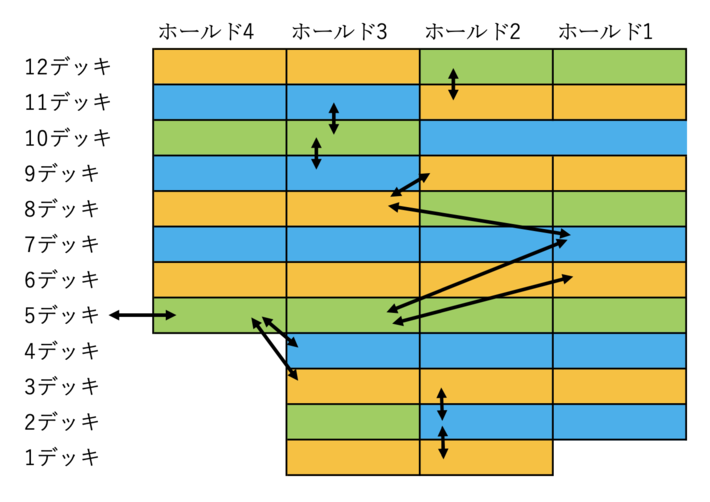
\includegraphics[slace=0.2]{segment.png}
 \caption{統合後のホールドを色付けしたもの}
 \label{fig1}
\end{figure}



\section{解の表現方法}
鵜川らによる研究の数理モデル\cite{ukawa}では,ホールドに注文を何台割り当てる,という連続的な解の表現方法を用いていた.
ヒューリスティックを用いるモデルでは,このような連続的な解表現方法を用いず,注文のセグメントへの割当のみを最適化し,詳細な車両の積載は決め打ちのルールを基に行っていく.
積載のルールは,ホールドの積載可能量,許容充填率などを満たすように設計を行っていく.

このように積載貨物を決めていくことで,注文を複数のホールドに渡って分割する場合であっても,隣接したホールドに車両を積むことができるため,プランナーの考える席割に近い解を出力することができる.

\section{局所探索法}
局所探索法とは, ある解に少しの変更を加え得た近傍解が元の解よりも良い解である場合に, 変更後の解に移動するという操作を良い解が見つからなくなるまで繰り返す方法である.
変形を加える操作を近傍操作と呼び, 近傍内に改善解を持たない解を局所最適解と呼ぶ.

本研究では,初期解を生成した後に局所探索法を用いて解の改善を行う手法を提案する.
また,評価関数として鵜川ら\cite{ukawa}によって提案された目的関数を用いる.
また,貨物の重量バランスに関する制約などに違反している場合には,制約違反度合いをペナルティ関数として表し, 目的関数に加えて探索を行う.

\section{初期解の生成}
\label{initial}
局所探索における初期解の生成方法として,2種類のアプローチを提案する.
\subsection{整数計画問題の緩和解の利用}
\label{relaxation}
定式化を行った整数計画問題の整数制約を緩和した線形緩和問題の解を初期解として利用することを考える.
この手法は,有効な解が得られたことが確認できている整数計画問題の解と線形緩和問題の性質が似ている場合に有効であると考えられる.
予備実験としてマンハッタン距離を用いてそれぞれの解の性質を比較する.

\subsubsection{マンハッタン距離}
マンハッタン距離とは,2点間の距離がどの程度離れているかを示すものである.

平面状の座標に置かれた点に対して,マンハッタン距離$d_1$は一般的に以下のように定義される.
\begin{align*}
 d_1(x,y) =\sum_{i=1}^n |x_i-y_i|
\end{align*}

\subsubsection{マンハッタン距離の計算方法}
本研究では,各注文におけるホールドへの割当台数を目的変数としている.
各注文における車両台数は異なるため,マンハッタン距離を計算するためには正規化をする必要がある.

注文における車両台数のなかで,特定のホールドに割り当てる注文台数の割合を変数とすると,0から1の値を必ずとることがわかる.
各注文において,注文が全て割り当てられていれば和は1になる.

整数計画問題の解と線形緩和問題の解をそれぞれ正規化したベクトルを$x,y$とする.
注文数を$n$,ホールドの数を$m$としたとき,マンハッタン距離を以下のように計算する.
\begin{align*}
 d_1(x,y) =\sum_{i=1}^n \sum_{j=1}^m|x_{ij}-y_{ij}|
\end{align*}
注文の全てが割り当てられている場合にマンハッタン距離の和は$2n$になるため,$2n$で割ると2つの解の性質がどの程度異なるかを測ることができる.


\subsubsection{線形緩和問題の解の性質}
整数計画問題の解と線形緩和問題の性質の比較を行う.
解の精度が十分に良いことがわかっている解で比較を行う必要があるため,整数計画問題において厳密解が出た問題例で比較を行い,結果を表\ref{hamming}に示す.

どの問題例においても,整数計画問題の解の性質に近い線形緩和問題の解が存在することが確認できた.

\begin{table}[h]
  \centering
  \caption{線形緩和問題の解との比較}
  \label{hamming}
\begin{tabular}{cccr}
\hline
注文数 & 積み地 & 揚げ地 & \multicolumn{1}{c}{解の差異(\%)} \\ \hline
38 & 2   & 3   & 0.19                        \\
63 & 2   & 3   & 3.57                         \\
57 & 2   & 5   & 1.07                         \\
66 & 4   & 3   & 0.71                        \\ \hline
\end{tabular}
\end{table}

\subsubsection{線形緩和解の丸め方}
線形緩和問題では,注文のホールドへの割当として小数点が出てくる場合がある.
各注文を,緩和解の変数値の最も大きいホールドに割り当てると一部のホールドに大量に割り当てられる解が出る可能性があるため,割り当てられた値を確率として,その確率を基にランダムに割り当てる手法で初期解を生成する.
ただし,割り当てるホールドの容量制約が満たされない場合には,そのホールドには割り当てない.


\subsection{港が同じ注文をまとめて席割を作成}
\label{model2}
鵜川らは,注文の積み地と揚げ地が同じ注文を1つのグループとして考え,グループ化された注文をホールドに割り当てることで計算時間を短縮する手法を提案した\cite{ukawa}.
解の精度としては,ある程度有効ではあるものの,実際に利用するためには修正が必要であった.

本研究では,この手法で得られた解を局所探索における初期解として利用するアプローチを提案する.


\section{近傍操作}
近傍操作には挿入近傍操作と交換近傍操作を用いる.

挿入近傍操作は,セグメントに割り当てられている注文の1つを,ランダムに異なるセグメントに挿入する操作である.
交換近傍操作は,異なるセグメントに割り当てられている注文を2つランダムに選び,それらを入れ替える操作である.

本研究では,はじめに挿入近傍操作を改善がなくなるまで繰り返し,その後交換近傍操作を改善がなくなるまで行う.
交換近傍操作で1回でも改善があった場合は,再び挿入近傍操作からやり直す.


\subsection{計算時間の短縮}
\label{近傍操作の計算時間短縮}
本研究では,局所探索における近傍操作の1つとして挿入近傍操作を用いるが,操作に工夫を加えることで解の精度を変化させることなく計算時間を短縮させることができると考えられる.

挿入近傍操作では,1つの注文を異なるセグメントに挿入する.その際に,挿入可能な位置すべてを探索し評価関数の値が最も良くなる位置に挿入する.

しかし,あるセグメントに格納される注文の順番が変化しても評価関数の値が全く変化しない場合がある.そのような場合にはすべての挿入可能位置を探索する必要がないため,計算時間を短縮することができる.

以下に計算時間を短縮する提案手法の概要を示す.

\begin{algorithm}
 \caption{計算時間を短縮する手法}
 \label{algo1}
 \begin{algorithmic}[1]%1を0にすると行番号なし.
  \STATE あるセグメントから,注文を1つ選択する
  \STATE 挿入先のセグメントの,一番最後の位置に挿入する
  \STATE 複数のセグメントに分割された注文を$J_{\rm split}$とする.
  \FOR {$j \in J_{\rm split}$}
  \STATE $j$の前後に注文を挿入する
  \IF {評価関数の値が暫定解よりも良い}
  \STATE 暫定解を更新
  \ENDIF
  \ENDFOR
  \IF {暫定解が探索における最良解よりも良い}
  \STATE 最良解を更新
  \ENDIF
 \end{algorithmic}
\end{algorithm}

\chapter{計算実験}\label{computational_result}
\section{実験環境}
実験に用いるプログラムは Pythonを用いて実装し, 計算機はPowerEdge T320 (CPU: Intel(R) Xeon(R) CPU E5-1410 v2 (2.80 GHz, 10 M cache), RAM: 96 GB) を使用した. また,整数計画ソルバーとしてGurobi Optimizer (ver 9.0.0) を使用した.

\section{計算時間の短縮}
\ref{近傍操作の計算時間短縮}で解の精度を変化させることなく計算時間を短縮する手法を提案した.
計算実験を行い,挿入可能な位置にすべて挿入した場合と提案手法において,計算時間の秒数の比較を行う.

挿入近傍操作を一定回数行った際の計算時間の比較結果を表\ref{shift}に示す.

提案手法により、全てのインスタンスにおいて計算時間が短縮できることを確認した.解の精度を落とすことなく計算時間を短縮することができるため,有効な手法だと考えられる.

\section{初期解による比較}
\label{sectioninitial}
\ref{initial}章で提案した初期解生成の手法と,注文をランダムに割り当てた初期解の比較を行う.
\ref{relaxation}章の緩和解を用いる方法を手法1,\ref{model2}章の港ごとに注文をまとめる方法を手法2,初期解をランダムに生成する方法を手法3と記す.計算結果を表\ref{initialresult}に示す.

結果より,手法1では線形緩和問題を解くことに多くの計算時間を要しており,初期解を生成するために計算時間を使いすぎていることが確認できた.
その一方で,ランダムに初期解を生成した場合には,比較的短い計算時間で,ある程度の精度の解を得る事ができることを確認した.


\section{2つの提案手法の比較}
\ref{method2}章で提案したヒューリスティックを用いる手法と,整数計画問題として解いた結果の比較を行う.
整数計画問題を解く手法では,探索を行って1時間後と24時間後の評価関数の値を記す.
ヒューリスティックを用いる手法では,\ref{sectioninitial}章で確認した最も解の精度が良い手法を記す.

結果より,計算時間を短縮しつつ,ある程度の精度の解を得ることができていることが確認できた.

\begin{table}[]
  \centering
  \caption{近傍操作に関する計算時間の比較}
  \label{shift}
\begin{tabular}{cccrr}
\hline
注文数 & 積み地 & 揚げ地 & \multicolumn{1}{c}{\begin{tabular}[c]{@{}c@{}}全ての位置\\ を探索\end{tabular}} & 提案手法 \\ \hline
109 & 2   & 3   & 145                                                                      & 81                        \\
109 & 2   & 5   & 192                                                                      & 89                        \\
109 & 4   & 3   & 122                                                                      & 99                        \\
250 & 2   & 3   & 387                                                                      & 204                       \\ \hline
\end{tabular}
\end{table}

\begin{table}[]
  \centering
  \caption{初期解生成による計算時間と解の比較}
  \label{initialresult}
\begin{tabular}{cccrrrrrr}
\hline
\multicolumn{3}{c}{問題例}                                                                               & \multicolumn{2}{c}{手法1}                          & \multicolumn{2}{c}{手法2}                          & \multicolumn{2}{c}{手法3}                          \\ \hline
注文数 & \begin{tabular}[c]{@{}c@{}}積み\\ 地\end{tabular} & \begin{tabular}[c]{@{}c@{}}揚げ\\ 地\end{tabular} & \multicolumn{1}{c}{計算時間} & \multicolumn{1}{c}{解} & \multicolumn{1}{c}{計算時間} & \multicolumn{1}{c}{解} & \multicolumn{1}{c}{計算時間} & \multicolumn{1}{c}{解} \\ \hline
109 & 2                                              & 3                                              & 1641                     & -2179                 & -                        & -                     & 873                      & -2975                 \\
109 & 2                                              & 5                                              & 8057                     & -594                  & -                        & -                     & 938                      & -1167                 \\
109 & 4                                              & 3                                              & 8782                     & 1840                  & -                        & -                     & 728                      & -1378                 \\
250 & 2                                              & 3                                              & 9726                     & -2755                 & -                        & -                     & 3069                     & -2235                 \\ \hline
\end{tabular}
\end{table}


\begin{table}[]\caption{提案手法による比較}
\centering
\label{heuristic}
\begin{tabular}{cccrrrr}
\hline
\multicolumn{3}{c}{問題例}                                                                               & \multicolumn{2}{c}{整数計画問題の解}                             & \multicolumn{2}{c}{ヒューリスティック}                    \\ \hline
注文数 & \begin{tabular}[c]{@{}c@{}}積み\\ 地\end{tabular} & \begin{tabular}[c]{@{}c@{}}揚げ\\ 地\end{tabular} & \multicolumn{1}{c}{1時間後の解} & \multicolumn{1}{c}{24時間後の解} & \multicolumn{1}{c}{計算時間} & \multicolumn{1}{c}{解} \\ \hline
109 & 2                                              & 3                                              & -508                       & -3478                       & 873                      & -2975                 \\
109 & 2                                              & 5                                              & -2612                      & -3354                       & 938                      & -1167                 \\
109 & 4                                              & 3                                              & 1240                       & -3455                       & 728                      & -1378                 \\
250 & 2                                              & 3                                              & 実行不可能                      & -2064                       & 3069                     & -2235                 \\ \hline
\end{tabular}
\end{table}

\chapter{まとめ}\label{conclution}
自動車運搬船における自動車を船に割り当てる席割の作成に関して,プランナーやオペレータとのヒアリングを基に定式化を行い2つの数理モデルを提案した.

整数計画ソルバーを用いて問題を解く際に,有効な解を出力することのできる問題例の規模を確認した.また,注文数が増えた場合や更なる制約や目的関数を追加する場合に計算時間が膨大に増大しないことを目指し,ヒューリスティックを用いた新たな数理モデルを提案した.

新たに提案した数理モデルの局所探索における近傍操作に関して,挿入近傍操作において解の精度を落とすことなく計算時間を短縮する手法を提案し,有効性を確認した.
また,局所探索における初期解を生成する手法を2種類提案し,計算実験を行い比較を行った.港ごとに注文をまとめて初期解を生成したのちに局所探索法を用いて解を改善することで, より短時間で精度の良い解を出力することを確認した.

ヒューリスティックを基にした新たな数理モデルを用いることで,整数計画問題を解く手法と比較して,計算時間を短縮しつつ精度の良い解を得ることができることを確認した.

\chapter*{謝辞}
お世話になった先生方に言葉では伝えきれないほどの感謝の念を伝えましょう. 
本研究の遂行にあたり, 熱心な指導と助言を頂きました柳浦睦憲教授に深く感謝の意を表します. 
提案手法の検討やその有用性において活発に議論を頂きました, 橋本英樹准教授, 胡艶楠氏, 呉偉氏に大変お世話になりました. 深くお礼申し上げます. 
日々の研究室生活においては柳浦研究室の皆様にお世話になりました. 
夜を徹して行った麻雀ではその最適戦略の見極めるために大変有意義なものでした. 
卒業旅行を楽しみにしています. 
皆様のおかげで有意義な研究活動に勤しむことができました. 深くお礼申し上げます. 





\addcontentsline{toc}{chapter}{参考文献}
\begin{thebibliography}{99}
  \bibitem{mitsui}
 「商船三井 プレスリリース」https://www.mol.co.jp/pr/2019/19072.html \\ (2020年11月24日)
 \bibitem{stowage}
 「日本橋海運 貿易関連用語集」http://nihonbashi-shipping.co.jp/lexicon/50\_su/
\bibitem{ukawa} 鵜川知哉, 自動車運搬船における貨物積載プランニングの席割問題に対する数理モデリング, 修士論文,名古屋大学情報学研究科, 2020
\bibitem{balance}
Eivind Wathne, Cargo Stowage Planning in RoRo Shipping, Master thesis, Norwegian University of Science and Technology, Marine Technology, 2012.
\end{thebibliography}
\end{document}



% LocalWords:  ij Imahori Yagiura Ibaraki th Metaheuristics McGeoch Aarts lrr
% LocalWords:  Lenstra Chichester algorithmicx Fulkerson lrrcrr
%%presented by YUKI SAWAI 2015/12/22
%この卒論修論はhttp://www.co.cm.is.nagoya-u.ac.jp/~yagiura/writing/haifu_template/をもとに澤井佑樹が作っています
